\documentclass[conference,onecolumn]{IEEEtran}
\usepackage{setspace}
\onehalfspacing
\usepackage{acronym}
\usepackage[backend=bibtex]{biblatex}
\usepackage{graphicx}
\usepackage{hyperref}
\usepackage[margin=3cm]{geometry}
\usepackage[english]{babel}

\addbibresource{../master-thesis.bib}

\begin{document}

  \title{Scientific Work: Creating a web-based model transformation UI (with GLSP)}

  \author{\IEEEauthorblockN{Florian Weidner}
    \IEEEauthorblockA{Philipps-University Marburg, Germany\\
      Department of Mathematics and Computer Science, Software engineering group\\
      May 06, 2025\\
  }}

  \maketitle

  \IEEEpeerreviewmaketitle

  \newpage

  \section{Motivation and introduction}
  \label{sec:motivation}

  In software engineering, often \ac{mde} is used to increase development productivity and quality. Concepts are modeled closer to the domain, so that they describe important aspects of a solution with human-friendly abstractions. The models can also be used to generate application fragments, that can be directly used as source code. In the process of \ac{mde}, many activities need to transform source models into different target models, while following a set of transformation rules. This model transformation process is based on algebraic graph transformations. A metamodel is used to model the structure and rules of the concept. The resulting transformation language can provide automatic model creation, development and maintenance activities. \cite{transformations-modeldriven} One framework to use \ac{mde} is \ac{emf} by the Eclipse Foundation. It provides a basis for application development, using modeling and code generation facilities. Much frameworks build upon \ac{emf}, providing various \ac{mde} tools like code generators, graphical diagramming, model transformation or model validation. \cite{emf} One model transformation framework is Henshin. \cite{henshin-repo} It tries to provides model transformation capabilites with a high level of usability. \cite{henshin-usability} For metamodels it uses \ac{emf} Ecore files and for instance models \ac{emf} XMI files. The framework enables transformations on XMI instance files with a defined transformation language. It provides a graphical and textual syntax to create these transformation rules. \cite{henshin-repo} Henshin can be used as a eclipse plugin. Eclipse makes it easy to access, but especially for new users, the heavy editor makes the use of Henshin unintuitive.

  Therefore the goal exists to create a graphical option to use the Henshin model transformations without the overhead of the heavy eclipse editor. A web-based graphical editor would make the use of Henshin even more accessible and intuitive.

  \ac{glsp} is a open-source framework by the Eclipse Foundation to develop custom diagram editors for distributed web-applications. \cite{glsp-repo} It can be used in Eclipse Desktop IDE, Eclipse Theia, Visual Studio Code and embedded in any website. With these fuctionalities, \ac{glsp} fits to create an accessible, intuitive application to create and apply Henshin model transformations.





  \section{Background}
  \label{sec:background}
  In this section, the theoretical background of the project and used technologies are described. 

  \subsection{Eclipse Foundation}
  \label{subsec:eclipse-foundation}
  The Eclipse Foundation is a not-for-profit, member-supported corporation that provides an environment for individuals and organizations for collaborative and innovative software development. \cite{eclipse-review} The Eclipse Foundation grew out of the publication of the Eclipse \ac{ide} code from IBM in 2001. The Eclipse Foundation itself was founded in 2004. The new organization was founded to continue the development of Eclipse IDE as an open source platform. Over time many different projects were initiated by the organization in the Eclipse environment, all running under the Eclipse Public License. \cite{heise-eclipse-foundation,eclipse-review} In the recent years, the key initatives of the Eclipse Foundation are contributing to european digital souvereignty, enhancing security measures, innovating \ac{sdv}, organizing community events and improving their most popular projects. Popular projects are for example the Jakarta EE, a ecosystem for cloud native applications with java, Eclipse Temurin, providing open source Java Development Kits and the Eclipse IDE. \cite{eclipse-report} In total, the Eclipse Foundation hosts more than 400 open source projects, supported 14 european research projects in 2024 and has 117 organisations participating in commits \cite{eclipse-report}

  The scope of this work remains within the Eclipse Foundation ecosystem. All frameworks used are projects from the Eclipse Foundation. The used frameworks are described in the sections \ref{subsec:emf}, \ref{subsec:henshin} and \ref{subsec:glsp}.

  The Eclipse \ac{ide} is not the main project but it is still an important part of the Eclipse infrastructure. It is divided into four main components: Equinox, the Platform, the \ac{jdt} and the \ac{pde}. Together they provide everything to develop and extend Eclipse-based tools. Equinox and the Platform are the core of the Eclipse \ac{ide}. With expanding the core with the \ac{jdt} or other plugins, the \ac{ide} can be used to develop different programming languages, like Java, C/C++ or PHP. \cite{emf} Eclipse provides different packages to download, depending on the use case. One package is the Eclipse Modeling Tools package by the Eclipse Modeling Project. It provides tools and runtimes to build model-based applications. It can be used to graphically design domain models and test those models by creating and editing dynamic instances. Also Java code can be generated from the models to get a scaffold, that can be used to create application on top. \cite{eclipse_modeling} The base of the Eclipse Modeling Tool is \ac{emf} (section \ref{subsec:emf}). Other modeling tools and projects, that are built on top of the \ac{emf} core functionality, provide capabilites for model transformation, database integration, or graphical editor generation. \cite{emf}

  \subsection{\acf{emf}}
    \label{subsec:emf}

    \begin{quote}
      \glqq\acf{emf} is a modeling framework and code generation facility for building tools and other applications based on a structured data model.\grqq{} \autocite{emf-repo}
    \end{quote}

    \acfi{emf} is the core part of the Eclipse Modeling Project and unifies the representation of models in \acs{uml}, \acs{xml} and Java. You can define your model in one of these formats and use \ac{emf} to generate the other formats.
    
    \ac{emf} consists of three components. The \ac{emf} core part, provides Ecore meta models, a runtime support for the models, and a basic \acs{api} for manipulating \ac{emf} objects generically. Ecore meta models are used to describe the structure of a model. \cite{eclipse_emf} They can be serialized in \ac{xmi} 2.0, as Ecore \ac{xmi} and have the file extension \textit{.ecore}. There are several Ecore classes to represent a model, here are the most important ones:

    \begin{itemize}
      \item \textbf{EClass}: A class in the model that is identified by a name, containing attributes and references to other classes. It can also refer to a number of other classes as its supertypes to support inheritance.\cite{emf}
      \item \textbf{EAttribute}: An attribute of a class, that are identified by a name and have a type.\cite{emf}
      \item \textbf{EDataType}: A simple data type like \textit{EString}, \textit{EBoolean} or \textit{EJavaClass}\cite{emf}
      \item \textbf{EReference}: A reference to another class, containing a link to an instance of that class.\cite{emf}
    \end{itemize}


    Together \citeauthor{emf} called these classes the Ecore kernel. In figure \ref{fig:emf-kernel} you can see the kernel classes and their relations. these classes are enough to define simple models. \textbf{EAttribute} and \textbf{EReference} have a lot of similarities. They both define the state of an instance of an \textbf{EClass} and have a name and a type. For that Ecore provides a common interface for both, called \textbf{EStructuralFeature}. Ecore can also model behavioral features of classes as \textbf{EOperation} using \textbf{EParameter}.
    Related classes are grouped into packages called \textbf{EPackage}. It is represented by the root element when the model is serialized. \cite{emf}

    \begin{figure}[h]
      \centering
      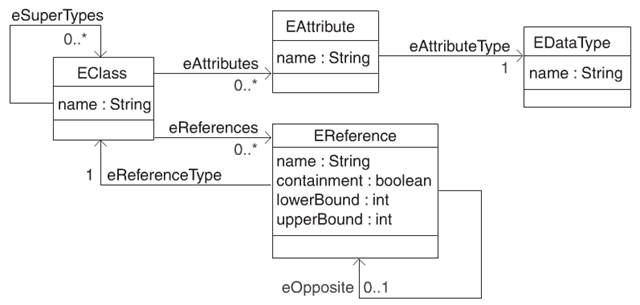
\includegraphics[width=0.7\textwidth]{figures/emf-kernel}
      \caption{The Ecore kernel. Image obtained from \cite{emf}}
      \label{fig:emf-kernel}
    \end{figure}

    The second component of \ac{emf} is \ac{emf}.Edit. It provides generic reusable classes to build viewers and editors for \ac{emf} models. With these classes \ac{emf} meta models can be displayed in JFace viewers, that are part of the Eclipse \acs{ui}. \cite{eclipse_emf} The Eclipse \ac{ide} can display a Ecore model in a tree viewer. Eclipse acceses the data over the \textit{ITreeContentProvider} interface to navigate the content and the\textit{ILabelProvider} interface to provide the label text and icons for the displayed objects.  The properties of objects are displayed in a Property Sheet over the \textit{IPropertySourceProvider}, where the user can edit the model.  \ac{emf}.Edit also provides undo and redo operations when creating or editing a instance model. For that it uses a command framework with commands like a \textit{AddCommand}, \textit{SetCommand} or \textit{CopyCommand}. \cite{emf}

    The third component is \ac{emf}.Codegen. It can generate Java code for a complete editor for \ac{emf} instance models of a Ecore meta model. It provides different generation options. So unlike \ac{emf}.Edit, that just provides generic classes for Ecore models, \ac{emf}.Codegen directly generates complete editors with a \acs{ui}. \cite{eclipse_emf} The generation can be done over a wizard in the Eclipse \ac{ide} or by using the command line interface. \cite{emf} The generation can be sepertated in to three levels. The first level is to generate Java interfaces and implementations for the Ecore model classes and a factory and package implementation class. The second level generates specific \textit{ItemProviders} to edit instance models based on the meta model.The classes are structured like the \ac{emf}.Edit component for the Ecore models. The third level generates a structured editor with \acs{ui} that works like the Ecore editor in the Eclipse \ac{ide} and can be a starting point for customization. \cite{eclipse_emf}

  \subsection{Henshin}
  \label{subsec:henshin}

  One part of the Eclipse Modeling Project for model transformation is Henshin. It can be used as a plugin in the Eclipse \ac{ide} or as an \acs{sdk}. It provides a graphical and textual syntax to define model transformation rules and apply them on \ac{emf} XMI instance models. It can be used for endogenous transformations, where \ac{emf} model instances are directly transformed, and exogenous transformations, where new instances are generated from given instances using a trace model. It also brings efficient in-place execution of transformations using a interpreter with debugging support and a performance profiler. Henshin also provides confilct and dependency analysis, and state space analysis for verification. \cite{henshin-repo}


  \subsection{\ac{glsp}}
  \label{subsec:glsp}

  \ac{glsp} is a framework that provides components for the development of \acsp{gui} for web-based diagram editors.
  \cite{glsp-repo}

  \section{Related Work/Software}
  \label{sec:related-work}

  Similar already existing tools for model checking: Henshin, Groovy...

  % \section{Project}
  % \label{sec:project-plan}

  % \subsection{Requirements}
  % \label{subsec:requirements}

  \subsection{Implementation}
  \label{subsec:implementation}


  \section{Conclusion}

  \printbibliography

  \newpage
  \section{Acronyms}
  \label{sec:acronyms}

  \begin{acronym}
    \acro{glsp}[GLSP]{Graphical Language Server Platform}
    \acro{emf}[EMF]{Eclipse Modeling Framework}
    \acro{mde}[MDE]{Model-Driven Engineering}
    \acro{ui}[UI]{User Interface}
    \acro{gui}[GUI]{Graphical \acf{ui}}
    \acro{ide}[IDE]{Integrated Development Environment}
    \acro{sdv}[SDV]{Software-Defined Vehicle}
    \acro{jdt}[JDT]{Java Development Tools}
    \acro{pde}[PDE]{Plug-in Development Environment}
    \acro{sdk}[SDK]{Software Development Kit}
    \acro{api}[API]{Application Programming Interface}
    \acro{uml}[UML]{Unified Modeling Language}
    \acro{xmi}[XMI]{XML Metadata Interchange}
    \acro{xml}[XML]{Extensible Markup Language}
    \acroplural{gui}[GUIs]{\ac{gui}s}
  \end{acronym}

\end{document}
